\chapter{Models on the Hourly Consumption}
In this section, a more detailed look at the hourly consumption will be provided. One of the goals is to get a better understanding of the tap-water consumption during the summer period, such that it can be used when looking at the winter period. This can be done by looking at the distributions of the consumption during the day in the two periods. Another goal of this section is to model the hourly consumption as a time series. An ARIMAX model will be applied to give a better understanding of the data. The ARIMAX model can also be used to give short term predictions of the consumption. These predictions will be compared to the ones provided by the multiple regression model.

\noindent \cref{fig: Hourcons_summer} and \cref{fig: Hourcons_winter}



\begin{figure}
    \centering
    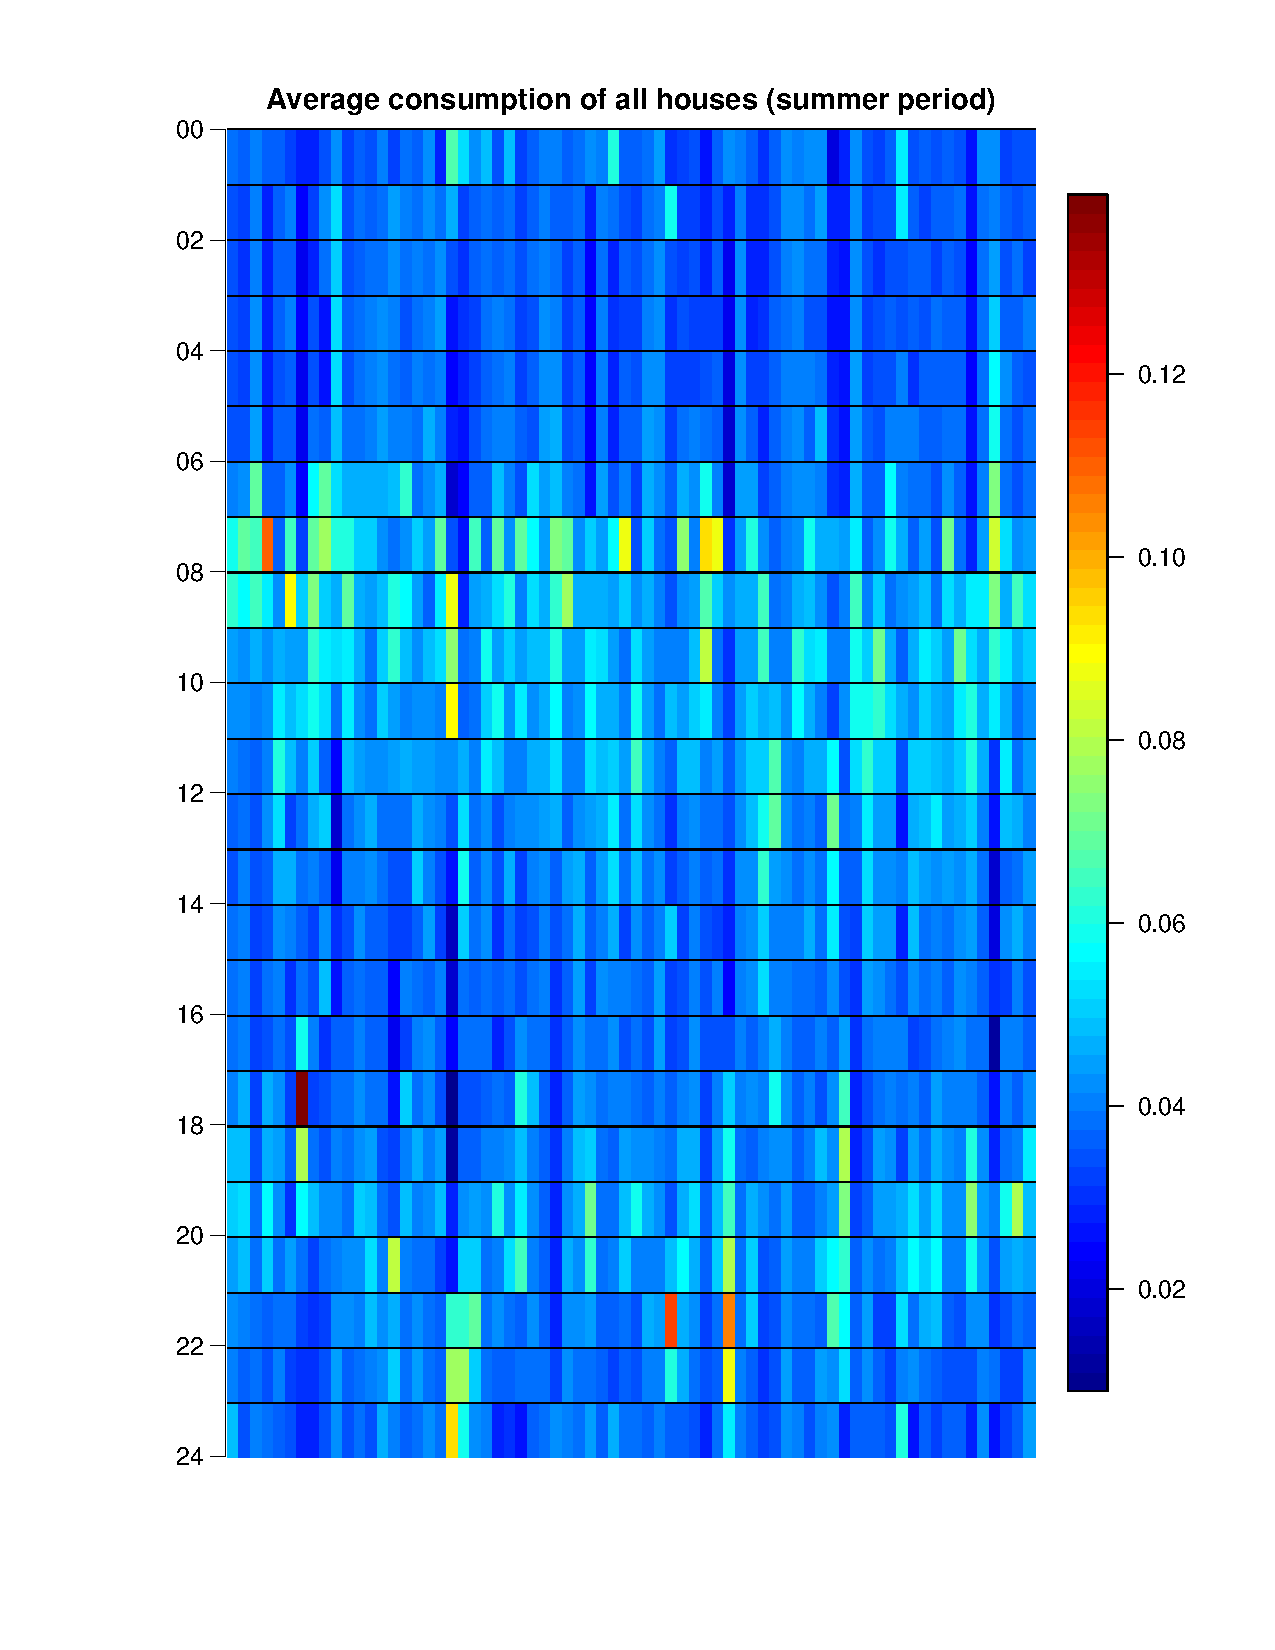
\includegraphics[width=\textwidth]{../../../figures/Heatmap_summer.pdf}
    \caption{The normalized average consumption of every house during the day in the summer period. This is characterized by the days where the average temperature is above 15 degrees. The horizontal lines indicate the hours and each vertical strip is a house. The scale indicates the fraction of the total consumption during the day}
    \label{fig: Hourcons_summer}
\end{figure}


\begin{figure}
    \centering
    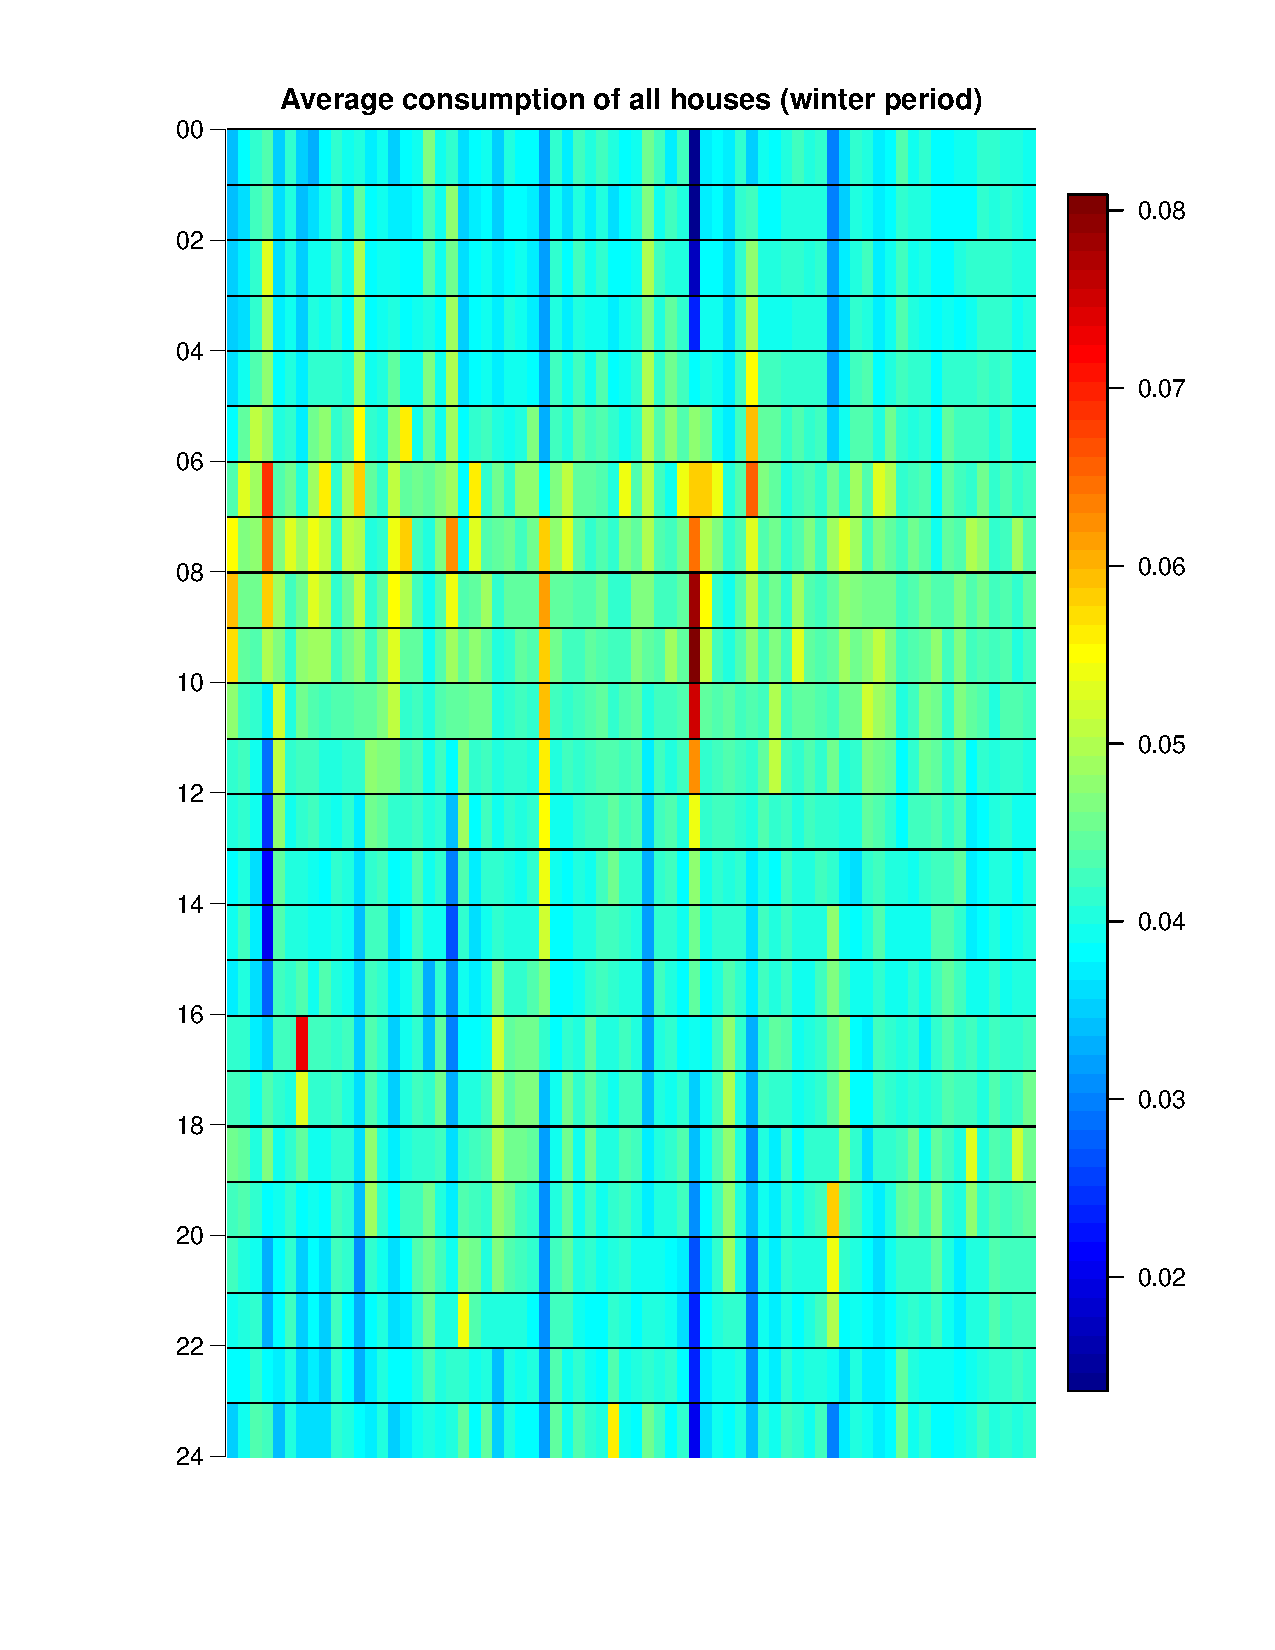
\includegraphics[width=\textwidth]{../../../figures/Heatmap_winter.pdf}
    \caption{This figure shows the same as \cref{fig: daily_cons}, but only in the winter period, characterized by a temperature below 12 degrees}
    \label{fig: Hourcons_winter}
\end{figure}







\section{ARIMAX}
An ARIMAX model is constructed for the hourly data of every house. The outside temperature is used as the exogenous variates. The exploratory analysis has shown that there is a high covariance between the temperature and the consumption, making this the obvious choice. The model is expected to have a seasonal component with season 24, because the consumption in certain time periods are likely to be close to each other from day to day.

\noindent In the following a general modelling approach will be used where a large model is applied at first. It is then reduced by looking at the standard deviation of the estimates on all houses. The initial model is an ARIMAX(2,2,2) model with a seasonal (0,1,1) component. This is a very extensive model, and differencing is used to make it stationary. \cref{arimax1_55} shows an example of how the model performs on house $55$, while \cref{arimax1_18} shows the same model for house $18$. For house $18$ both the ACF and the PACF ressemble white noise fairly well, with a few exceptions. The same goes for house $55$. Both have a few significant lags, and they both have a significant lag around lag $61$, even though it is barely so. It is supricing that neither house have lags in the seasons that are even close to being significant. This indicates that the dependencies from day to day might not be as important as it was initially assumed. But as mentioned, this model has some parameters that might not be necessary to include.




\begin{figure}
    \centering
    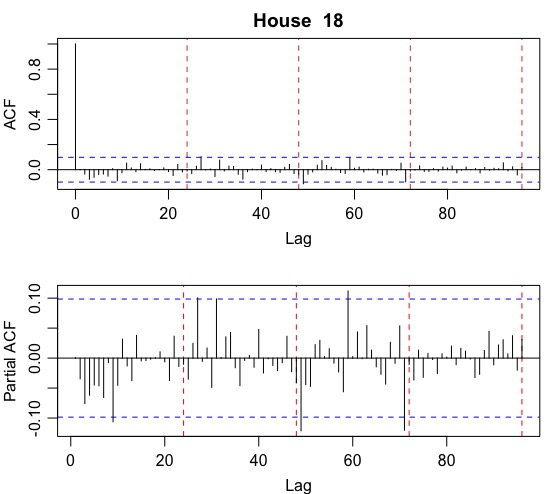
\includegraphics[width=0.8\textwidth]{../../../figures/arimax/Arimax1_18.jpeg}
    \caption{The autocorrelation function for the ARIMAX(2,2,2)$\times$(0,1,1) model, based on the data from house 18}
    \label{arimax1_18}
\end{figure}


\begin{figure}
    \centering
    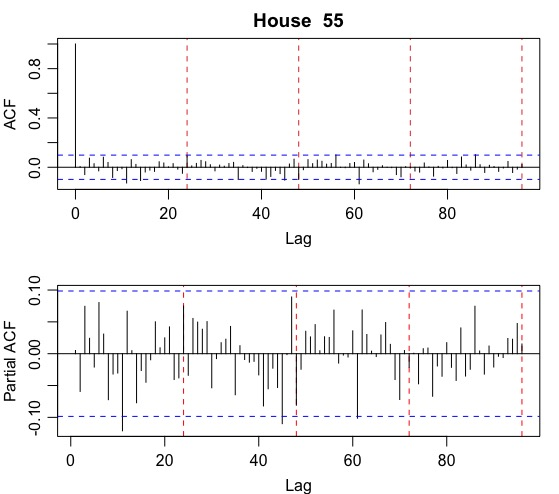
\includegraphics[width=0.8\textwidth]{../../../figures/arimax/Arimax1_55.jpeg}
    \caption{The partial autocorrelation function for the ARIMAX(2,2,2)$\times$(0,1,1) model, based on the data from house 18}
    \label{arimax1_55}
\end{figure}

\begin{table}[]
    \begin{tabular}{|l|l|l|l|l|l|l|l|}
    \hline
    Parameters     & AR1  & AR2  & MA1  & MA2  & SMA1 & Intercept & Temperature \\ \hline
    Insignificance & 24\% & 81\% & 15\% & 13\% & 0\%  & 0\%       & 3\%         \\ \hline
    \end{tabular}
    \caption{For each parameter in the first ARIMAX model, this table shows how many of the houses have an estimate that is less than two standard deviations. The average Log Likelihood of the model is $-77$}
    \label{First arimax}
    \end{table}

Der er ikke noget i lag 24. Seasonal er ret ligegyldigt.
ARIMAX er en del bedre end ARIMA med temperatur som covariate.
Vi kører en (1,0,1) model. De fleste ser fine ud. Men nogen har ret signifikante lags, specielt in pacf.
Derfor tilføjes ar(2) og ma(2). Der er mange forskellige modeller og i nogen er bestemte parametrer meget insignifikante.
Der kommer også warnings for nogen af dem.
qq-lines er fine for mange af modellerne, dårlige for nogen af dem.
Nogen huse er helt hen i vejret (Øv, hus 28). De har meget oscillering.
